% ******************************* PhD Thesis Template **************************
% Please have a look at the README.md file for info on how to use the template

\documentclass[a4paper,12pt,times,numbered,print,index]{Classes/PhDThesisPSnPDF}

% ******************************************************************************
% ******************************* Class Options ********************************
% *********************** See README for more details **************************
% ******************************************************************************

% `a4paper'(The University of Cambridge PhD thesis guidelines recommends a page
% size a4 - default option) or `a5paper': A5 Paper size is also allowed as per
% the Cambridge University Engineering Deparment guidelines for PhD thesis
%
% `11pt' or `12pt'(default): Font Size 10pt is NOT recommended by the University
% guidelines
%
% `oneside' or `twoside'(default): Printing double side (twoside) or single
% side.
%
% `print': Use `print' for print version with appropriate margins and page
% layout. Leaving the options field blank will activate Online version.
%
% `index': For index at the end of the thesis
%
% `draftclassic': For draft mode without loading any images (same as draft in book)
%
% `draft': Special draft mode with line numbers, images, and water mark with
% timestamp and custom text. Position of the text can also be modified.
%
% `abstract': To generate only the title page and abstract page with
% dissertation title and name, to submit to the Student Registry
%
% `chapter`: This option enables only the specified chapter and it's references
%  Useful for review and corrections.
%
% ************************* Custom Page Margins ********************************
%
% `custommargin`: Use `custommargin' in options to activate custom page margins,
% which can be defined in the preamble.tex. Custom margin will override
% print/online margin setup.
%
% *********************** Choosing the Fonts in Class Options ******************
%
% `times' : Times font with math support. (The Cambridge University guidelines
% recommend using times)
%
% `fourier': Utopia Font with Fourier Math font (Font has to be installed)
%            It's a free font.
%
% `customfont': Use `customfont' option in the document class and load the
% package in the preamble.tex
%
% default or leave empty: `Latin Modern' font will be loaded.
%
% ********************** Choosing the Bibliography style ***********************
%
% `authoryear': For author-year citation eg., Krishna (2013)
%
% `numbered': (Default Option) For numbered and sorted citation e.g., [1,5,2]
%
% `custombib': Define your own bibliography style in the `preamble.tex' file.
%              `\RequirePackage[square, sort, numbers, authoryear]{natbib}'.
%              This can be also used to load biblatex instead of natbib
%              (See Preamble)
%
% **************************** Choosing the Page Style *************************
%
% `default (leave empty)': For Page Numbers in Header (Left Even, Right Odd) and
% Chapter Name in Header (Right Even) and Section Name (Left Odd). Blank Footer.
%
% `PageStyleI': Chapter Name next & Page Number on Even Side (Left Even).
% Section Name & Page Number in Header on Odd Side (Right Odd). Footer is empty.
%
% `PageStyleII': Chapter Name on Even Side (Left Even) in Header. Section Number
% and Section Name in Header on Odd Side (Right Odd). Page numbering in footer

% Uncomment to change page style
%\pagestyle{PageStyleII}

% ********************************** Preamble **********************************
% Preamble: Contains packages and user-defined commands and settings
% ******************************************************************************
% ****************************** Custom Margin *********************************

% Add `custommargin' in the document class options to use this section
% Set {innerside margin / outerside margin / topmargin / bottom margin}  and
% other page dimensions
\ifsetCustomMargin
  \RequirePackage[left=37mm,right=30mm,top=35mm,bottom=30mm]{geometry}
  \setFancyHdr % To apply fancy header after geometry package is loaded
\fi

% Add spaces between paragraphs
%\setlength{\parskip}{0.5em}
% Ragged bottom avoids extra whitespaces between paragraphs
\raggedbottom
% To remove the excess top spacing for enumeration, list and description
%\usepackage{enumitem}
%\setlist[enumerate,itemize,description]{topsep=0em}

% *****************************************************************************
% ******************* Fonts (like different typewriter fonts etc.)*************

% Add `customfont' in the document class option to use this section

\ifsetCustomFont
  % Set your custom font here and use `customfont' in options. Leave empty to
  % load computer modern font (default LaTeX font).
  %\RequirePackage{helvet}

  % For use with XeLaTeX
  %  \setmainfont[
  %    Path              = ./libertine/opentype/,
  %    Extension         = .otf,
  %    UprightFont = LinLibertine_R,
  %    BoldFont = LinLibertine_RZ, % Linux Libertine O Regular Semibold
  %    ItalicFont = LinLibertine_RI,
  %    BoldItalicFont = LinLibertine_RZI, % Linux Libertine O Regular Semibold Italic
  %  ]
  %  {libertine}
  %  % load font from system font
  %  \newfontfamily\libertinesystemfont{Linux Libertine O}
\fi

% *****************************************************************************
% **************************** Custom Packages ********************************

% ************************* Algorithms and Pseudocode **************************

%\usepackage{algpseudocode}


% ********************Captions and Hyperreferencing / URL **********************

% Captions: This makes captions of figures use a boldfaced small font.
%\RequirePackage[small,bf]{caption}

\RequirePackage[labelsep=space,tableposition=top]{caption}
\renewcommand{\figurename}{Fig.} %to support older versions of captions.sty


% *************************** Graphics and figures *****************************

%\usepackage{rotating}
%\usepackage{wrapfig}

% Uncomment the following two lines to force Latex to place the figure.
% Use [H] when including graphics. Note 'H' instead of 'h'
%\usepackage{float}
%\restylefloat{figure}

% Subcaption package is also available in the sty folder you can use that by
% uncommenting the following line
% This is for people stuck with older versions of texlive
%\usepackage{sty/caption/subcaption}
\usepackage{subcaption}

% ********************************** Tables ************************************
\usepackage{booktabs} % For professional looking tables
\usepackage{multirow}

%\usepackage{multicol}
%\usepackage{longtable}
%\usepackage{tabularx}


% *********************************** SI Units *********************************
\usepackage{siunitx} % use this package module for SI units


% ******************************* Line Spacing *********************************

% Choose linespacing as appropriate. Default is one-half line spacing as per the
% University guidelines

% \doublespacing
% \onehalfspacing
% \singlespacing


% ************************ Formatting / Footnote *******************************

% Don't break enumeration (etc.) across pages in an ugly manner (default 10000)
%\clubpenalty=500
%\widowpenalty=500

%\usepackage[perpage]{footmisc} %Range of footnote options


% *****************************************************************************
% *************************** Bibliography  and References ********************

%\usepackage{cleveref} %Referencing without need to explicitly state fig /table

% Add `custombib' in the document class option to use this section
\ifuseCustomBib
   \RequirePackage[square, sort, numbers, authoryear]{natbib} % CustomBib

% If you would like to use biblatex for your reference management, as opposed to the default `natbibpackage` pass the option `custombib` in the document class. Comment out the previous line to make sure you don't load the natbib package. Uncomment the following lines and specify the location of references.bib file

%\RequirePackage[backend=biber, style=numeric-comp, citestyle=numeric, sorting=nty, natbib=true]{biblatex}
%\bibliography{References/references} %Location of references.bib only for biblatex

\fi

% changes the default name `Bibliography` -> `References'
\renewcommand{\bibname}{References}


% ******************************************************************************
% ************************* User Defined Commands ******************************
% ******************************************************************************

% *********** To change the name of Table of Contents / LOF and LOT ************

%\renewcommand{\contentsname}{My Table of Contents}
%\renewcommand{\listfigurename}{My List of Figures}
%\renewcommand{\listtablename}{My List of Tables}


% ********************** TOC depth and numbering depth *************************

\setcounter{secnumdepth}{2}
\setcounter{tocdepth}{2}


% ******************************* Nomenclature *********************************

% To change the name of the Nomenclature section, uncomment the following line

%\renewcommand{\nomname}{Symbols}


% ********************************* Appendix ***********************************

% The default value of both \appendixtocname and \appendixpagename is `Appendices'. These names can all be changed via:

%\renewcommand{\appendixtocname}{List of appendices}
%\renewcommand{\appendixname}{Appndx}

% *********************** Configure Draft Mode **********************************

% Uncomment to disable figures in `draft'
%\setkeys{Gin}{draft=true}  % set draft to false to enable figures in `draft'

% These options are active only during the draft mode
% Default text is "Draft"
%\SetDraftText{DRAFT}

% Default Watermark location is top. Location (top/bottom)
%\SetDraftWMPosition{bottom}

% Draft Version - default is v1.0
%\SetDraftVersion{v1.1}

% Draft Text grayscale value (should be between 0-black and 1-white)
% Default value is 0.75
%\SetDraftGrayScale{0.8}


% ******************************** Todo Notes **********************************
%% Uncomment the following lines to have todonotes.

%  \ifsetDraft
% 	\usepackage[colorinlistoftodos]{todonotes}
% 	\newcommand{\mynote}[1]{\todo[author=kks32,size=\small,inline,color=green!40]{#1}}
% \else
% 	\newcommand{\mynote}[1]{}
% 	\newcommand{\listoftodos}{}
% \fi



% ************************ Thesis Information & Meta-data **********************
% Thesis title and author information, refernce file for biblatex
% ************************ Thesis Information & Meta-data **********************
%% The title of the thesis
\title{Behavioral clues for forager transitions in a fully tracked honeybee colony}
%\texorpdfstring is used for PDF metadata. Usage:
%\texorpdfstring{LaTeX_Version}{PDF Version (non-latex)} eg.,
%\texorpdfstring{$sigma$}{sigma}

%% Subtitle (Optional)
% \subtitle{Using the CUED template}

%% The full name of the author
\author{Janek Szynal}

%% Department (eg. Department of Engineering, Maths, Physics)
\dept{Biorobotics Lab}

%% University and Crest
\university{Free University of Berlin}
% Crest minimum should be 30mm.
\crest{
\includegraphics[width=0.2\textwidth]{fu-crest}}
%% Use this crest, if you are using the college crest
%% Crest long miminum should be 65mm
%\crest{
\includegraphics[width=0.45\textwidth]{University_Crest_Long}}

%% College shield [optional] 
% Crest minimum should be 30mm.
%\collegeshield{\includegraphics[width=0.2\textwidth]{CollegeShields/Kings}}


%% Supervisor (optional)
%% for multiple supervisors, append each supervisor with the \newline command
\supervisor{Dr. Tim Landgraf}

%% Supervisor Role (optional) - Supervisor (default) or advisor
% \supervisorrole{\textbf{Supervisors: }}
%% if no title is desired:
% \supervisorrole{}

%% Supervisor line width: required to align supervisors
\supervisorlinewidth{0.35\textwidth}

%% Advisor (optional)
%% for multiple advisors, append each advisor with the \newline command
%\advisor{Dr. A. Advisor\newline
%Dr. B. Advisor}
     
%% Advisor Role (optional) - Advisor (default) or leave empty
% \advisorrole{Advisors: }
%% if no title is required
% \advisorrole{}

%% Advisor line width: required to align supervisors
%\advisorlinewidth{0.25\textwidth}


%% You can redefine the submission text:
% Default as per the University guidelines:
% ``This dissertation is submitted for the degree of''
%\renewcommand{\submissiontext}{change the default text here if needed}

%% Full title of the Degree
\degreetitle{Bachelor of Computer Science}

%% College affiliation (optional)
% \college{King's College}

%% Submission date
% Default is set as {\monthname[\the\month]\space\the\year}
%\degreedate{September 2014} 

%% Meta information
\subject{LaTeX} \keywords{{LaTeX} {PhD Thesis} {Engineering} {University of
Cambridge}}


% ***************************** Abstract Separate ******************************
% To printout only the titlepage and the abstract with the PhD title and the
% author name for submission to the Student Registry, use the `abstract' option in
% the document class.

\ifdefineAbstract
 \pagestyle{empty}
 \includeonly{Declaration/declaration, Abstract/abstract}
\fi

% ***************************** Chapter Mode ***********************************
% The chapter mode allows user to only print particular chapters with references
% Title, Contents, Frontmatter are disabled by default
% Useful option to review a particular chapter or to send it to supervisior.
% To use choose `chapter' option in the document class

\ifdefineChapter
 \includeonly{Chapter3/chapter3}
\fi

% ******************************** Front Matter ********************************
\begin{document}

\frontmatter

\maketitle

% ******************************* Thesis Dedidcation ********************************

\begin{dedication} 

I would like to dedicate this thesis to my loving parents \dots

\end{dedication}

% ******************************* Thesis Declaration ***************************

\begin{declaration}


I hereby declare that except where specific reference is made to the work of 
others, the contents of this dissertation are original and have not been 
submitted in whole or in part for consideration for any other degree or 
qualification in this, or any other university. This dissertation is my own 
work and contains nothing which is the outcome of work done in collaboration 
with others, except as specified in the text and Acknowledgements. 
\vspace{50pt}
\hrule
\vspace{50pt}
Ich versichere hiermit an Eides Statt, dass diese Arbeit von niemand anderem als meiner Person verfasst worden ist. Alle verwendeten Hilfsmittel wie Berichte, Bücher, Internetseiten oder ähnliches sind im Literaturverzeichnis angegeben, Zitate aus frem- den Arbeiten sind als solche kenntlich gemacht. Die Arbeit wurde bisher in gleicher oder ähnlicher Form keiner anderen Prüfungskommission vorgelegt und auch nicht veröffentlicht.
% Author and date will be inserted automatically from thesis.tex \author \degreedate

\end{declaration}
% ************************** Thesis Acknowledgements **************************

\begin{acknowledgements}      


And I would like to acknowledge ...


\end{acknowledgements}

% ************************** Thesis Abstract *****************************
% Use `abstract' as an option in the document class to print only the titlepage and the abstract.
\begin{abstract}
This is where you write your abstract ...
\end{abstract}


% *********************** Adding TOC and List of Figures ***********************

\tableofcontents

% \listoffigures

% \listoftables

% \printnomenclature[space] space can be set as 2em between symbol and description
%\printnomenclature[3em]

\printnomenclature

% ******************************** Main Matter *********************************
\mainmatter

%!TEX root = ../thesis.tex
%*******************************************************************************
%*********************************** First Chapter *****************************
%*******************************************************************************

\chapter{Introduction - 95\%}  %Title of the First Chapter

\ifpdf
    \graphicspath{{Chapters/Chapter1/Figs/Raster/}{Chapters/Chapter1/Figs/PDF/}{Chapters/Chapter1/Figs/}}
\else
    \graphicspath{{Chapters/Chapter1/Figs/Vector/}{Chapters/Chapter1/Figs/}}
\fi


%********************************** %First Section  **************************************
\section{The honeybee and the division of labor} %Section - 1.1 %TODO: is the title good?
%TODO: indent the first paragraph 
A honeybee (\textit{Apis mellifera}) colony manifests multiple fascinating examples of complex adaptive behaviour. 
Localized cues exchanged between individuals amount to emergent directional signals for the entire colony 
in ways heavily investigated, but often still not completely understood. 

One of the most notable and well-researched adaptive mechanisms of a colony is its division of labor (DOL). 
During the winter (a season of low activity for the bees), the colony focuses on survival 
and its workers are generalists, performing sets of tasks not easily distinguishable from those of other workers. 

For the spring-summer season, however, the hive’s goals change and along with them, the patterns of labor division. 
Hive growth and resource accumulation take priority, and specialization eventuates amongst workers. 
They begin to fill distinct roles, the allocation of which highly correlates with age (an effect 
known as temporal polyethism) - but is also grounded in the colony’s current needs and in environmental 
factors affecting it (adaptive behaviour) \citep{seeley_adaptive_1982}. Groups of workers that can be 
categorized as performing the same set of tasks are commonly referred to as castes. It is common to recognize 
four of them in the temporal caste system that the worker bees exhibit in the summer:
\textit{cell cleaners, nurses, middle-aged bees (MABs),} and \textit{foragers}. 
This work concentrates on the transition between \textit{MABs} and \textit{foragers}, 
possibly the most distinguishable and important in the lifecycle of a bee.


%********************************** %Second Section  **************************************
\section{The foraging phase}
The foraging phase is the last one in a bee’s life and comes with an increased risk of death. 
It is often proposed that this has to do with the extreme strain foraging puts on their bodies - 
essentially causing them to work themselves to death. This is supported for example by 
\citep{williams_age_2008}, % Williams, 2008 vs [3] 
who have shown honeybee flight to cause extremely high metabolic rates and induce oxidative stress, 
likely significantly accelerating the ageing process and causing early deaths. On the other hand,
the results of \citep{visscher_survivorship_1997} suggest that foragers’ deaths are usually caused 
not by senescence, but rather by the heightened risks of outside life that come with their function 
(such as the risk of predation). According to their findings, forager mortality rates are constant 
with respect to age - and not accelerating, as would have been suggested by the body strain hypothesis. 

Regardless of the reasons behind it, foraging nearly always ends in the death of a bee. That fact, 
combined with an estimate of the length of the foraging phase  (mean of 7.7 days ± 0.75 days, 
median of 7 days, and range of 2 to 17 day according to \citep{visscher_survivorship_1997}, 
should allow us to get a very simple estimate of the foraging period, which we can then use 
to validate the results we produce with more involved methods.
%TODO: make sure to indeed validate; or remove that claim

%TODO: cute tiny table with the data quoted above 


%********************************** %Third Section  **************************************
\section{The \textit{BeesBook} project}
This work operates on data from the 2016 iteration of the BeesBook project \citep{wario_automatic_2015}. 
A hard- and software framework is set up, allowing for high-confidence tracking of all individuals over 
the entire lifespan of a honeybee colony. It is the first dataset ever collected (to our knowledge) 
that is extensive enough to provide a comprehensive view of a hive’s life, maintaining the spatial, 
temporal and social context of the information it stores. 

The data it collects can be put in 3 categories: 
\begin{itemize}
    \item a list of detections (each assigned to a bee, a point in time and a point in the hive space) 
    \item a collection of individuals’ paths (added in [X])
    \item and a collection of bee waggle dance occurrences (added in [X]). 
\end{itemize}
%TODO: are paths separate or integrated: were they added later? what about dances?

The original \textit{BeesBook} paper put significant focus on waggle dance research, but the dataset and 
collection method is meant to serve a very general purpose. The system is described to be “conceived as 
a budget-priced framework for the incremental development of software and hardware components”, 
capable of supporting a wide range of investigations into invertebrates, the waggle dance, honeybee division 
of labor, collective intelligence and other related fields.



%********************************** %Fourth Section  **************************************
\section{This work's goals}
This work’s primary goal is to add building blocks to the \textit{BeesBook} project by deriving new abstractions
that can be used in future analyses and to show how the process of deriving such abstractions could look like.

A secondary goal is to provide an example of how analysis could be undertaken in the future, 
given the data, the set of abstractions and the process for creating them. 
%!TEX root = ../thesis.tex
%*******************************************************************************
%*********************************** Second Chapter *****************************
%*******************************************************************************

\chapter{Related work}  %"Related work and state of the art"?

\ifpdf
    \graphicspath{{Chapters/Chapter2/Figs/Raster/}{Chapters/Chapter2/Figs/PDF/}{Chapters/Chapter2/Figs/}}
\else
    \graphicspath{{Chapters/Chapter2/Figs/Vector/}{Chapters/Chapter2/Figs/}}
\fi

I present related work in three categories. The first one is an introduction to invertebrate tracking 
and automated observation, along with an overview of the state of the art. 

The second focuses on the division of labor in honeybees. It’s meant to set foundation for the analysis 
that we undertake in this work, as well as for determining what other kinds of approaches should be accessible 
given the BeesBook dataset and the building blocks that this work adds to it.

Finally, the last one collects works similar to this contribution - ones that use the \textit{BeesBook} 
dataset to perform some analysis of a honeybee colony’s life and/or add their own functionalities or improvements 
to the system.


%********************************** %First Section  **************************************
\section{Invertebrate observation and tracking} 

Observing invertebrates at scale, before a certain degree of automation was possible, required 
a lot of careful manual work and some creative approaches. A fascinating example of how experiments 
were conducted back then can be found in \citep{seeley_adaptive_1982}. The authors mark a hundred bees out of a 
colony of 21 thousand, using a brush with pigment mixed with shellac (following the example set 
by \citep{von_frisch_tanzsprache_1965}). They then pick for observation small subsections of the hive 
(quadrants), employing the help of a Texas Instruments calculator to generate randomness for their choices. 
Inferences about the entire population are made using the samples, but even to observe the samples, 8 hours 
of continuous work per day, for over 20 days, was necessary. To create maps of activity, authors used glass 
sheets that they put markings on and exchanged every day. They then photographed the sheets and projected the 
photographs against a single sheet of paper, one by one, thereby aggregating the one-day information sets 
into a single map. They also used a number of other physical and numerical tricks to 
be able to produce quality data. 


%********************************** %Second Section  **************************************



%********************************** %Third Section  **************************************



%********************************** %Fourth Section  **************************************

%!TEX root = ../thesis.tex
%*******************************************************************************
%****************************** Third Chapter **********************************
%*******************************************************************************
\chapter{My third chapter}

% **************************** Define Graphics Path **************************
\ifpdf
    \graphicspath{{Chapters/Chapter3/Figs/Raster/}{Chapters/Chapter3/Figs/PDF/}{Chapters/Chapter3/Figs/}}
\else
    \graphicspath{{Chapters/Chapter3/Figs/Vector/}{Chapters/Chapter3/Figs/}}
\fi

\section{First section of the third chapter}
And now I begin my third chapter here \dots

And now to cite some more people~\citet{Rea85,Ancey1996}

\subsection{First subsection in the first section}
\dots and some more 

\subsection{Second subsection in the first section}
\dots and some more \dots

\subsubsection{First subsub section in the second subsection}
\dots and some more in the first subsub section otherwise it all looks the same
doesn't it? well we can add some text to it \dots

\subsection{Third subsection in the first section}
\dots and some more \dots

\subsubsection{First subsub section in the third subsection}
\dots and some more in the first subsub section otherwise it all looks the same
doesn't it? well we can add some text to it and some more and some more and
some more and some more and some more and some more and some more \dots

\subsubsection{Second subsub section in the third subsection}
\dots and some more in the first subsub section otherwise it all looks the same
doesn't it? well we can add some text to it \dots

\section{Second section of the third chapter}
and here I write more \dots

\section{The layout of formal tables}
This section has been modified from ``Publication quality tables in \LaTeX*''
 by Simon Fear.

The layout of a table has been established over centuries of experience and 
should only be altered in extraordinary circumstances. 

When formatting a table, remember two simple guidelines at all times:

\begin{enumerate}
  \item Never, ever use vertical rules (lines).
  \item Never use double rules.
\end{enumerate}

These guidelines may seem extreme but I have
never found a good argument in favour of breaking them. For
example, if you feel that the information in the left half of
a table is so different from that on the right that it needs
to be separated by a vertical line, then you should use two
tables instead. Not everyone follows the second guideline:

There are three further guidelines worth mentioning here as they
are generally not known outside the circle of professional
typesetters and subeditors:

\begin{enumerate}\setcounter{enumi}{2}
  \item Put the units in the column heading (not in the body of
          the table).
  \item Always precede a decimal point by a digit; thus 0.1
      {\em not} just .1.
  \item Do not use `ditto' signs or any other such convention to
      repeat a previous value. In many circumstances a blank
      will serve just as well. If it won't, then repeat the value.
\end{enumerate}

A frequently seen mistake is to use `\textbackslash begin\{center\}' \dots `\textbackslash end\{center\}' inside a figure or table environment. This center environment can cause additional vertical space. If you want to avoid that just use `\textbackslash centering'


\begin{table}
\caption{A badly formatted table}
\centering
\label{table:bad_table}
\begin{tabular}{|l|c|c|c|c|}
\hline 
& \multicolumn{2}{c}{Species I} & \multicolumn{2}{c|}{Species II} \\ 
\hline
Dental measurement  & mean & SD  & mean & SD  \\ \hline 
\hline
I1MD & 6.23 & 0.91 & 5.2  & 0.7  \\
\hline 
I1LL & 7.48 & 0.56 & 8.7  & 0.71 \\
\hline 
I2MD & 3.99 & 0.63 & 4.22 & 0.54 \\
\hline 
I2LL & 6.81 & 0.02 & 6.66 & 0.01 \\
\hline 
CMD & 13.47 & 0.09 & 10.55 & 0.05 \\
\hline 
CBL & 11.88 & 0.05 & 13.11 & 0.04\\ 
\hline 
\end{tabular}
\end{table}

\begin{table}
\caption{A nice looking table}
\centering
\label{table:nice_table}
\begin{tabular}{l c c c c}
\hline 
\multirow{2}{*}{Dental measurement} & \multicolumn{2}{c}{Species I} & \multicolumn{2}{c}{Species II} \\ 
\cline{2-5}
  & mean & SD  & mean & SD  \\ 
\hline
I1MD & 6.23 & 0.91 & 5.2  & 0.7  \\

I1LL & 7.48 & 0.56 & 8.7  & 0.71 \\

I2MD & 3.99 & 0.63 & 4.22 & 0.54 \\

I2LL & 6.81 & 0.02 & 6.66 & 0.01 \\

CMD & 13.47 & 0.09 & 10.55 & 0.05 \\

CBL & 11.88 & 0.05 & 13.11 & 0.04\\ 
\hline 
\end{tabular}
\end{table}


\begin{table}
\caption{Even better looking table using booktabs}
\centering
\label{table:good_table}
\begin{tabular}{l c c c c}
\toprule
\multirow{2}{*}{Dental measurement} & \multicolumn{2}{c}{Species I} & \multicolumn{2}{c}{Species II} \\ 
\cmidrule{2-5}
  & mean & SD  & mean & SD  \\ 
\midrule
I1MD & 6.23 & 0.91 & 5.2  & 0.7  \\

I1LL & 7.48 & 0.56 & 8.7  & 0.71 \\

I2MD & 3.99 & 0.63 & 4.22 & 0.54 \\

I2LL & 6.81 & 0.02 & 6.66 & 0.01 \\

CMD & 13.47 & 0.09 & 10.55 & 0.05 \\

CBL & 11.88 & 0.05 & 13.11 & 0.04\\ 
\bottomrule
\end{tabular}
\end{table}

%!TEX root = ../thesis.tex
%*******************************************************************************
%*********************************** Fourth Chapter *****************************
%*******************************************************************************

\chapter{Evaluation}  %Title 

\ifpdf
    \graphicspath{{Chapters/Chapter4/Figs/Raster/}{Chapters/Chapter4/Figs/PDF/}{Chapters/Chapter4/Figs/}}
\else
    \graphicspath{{Chapters/Chapter4/Figs/Vector/}{Chapters/Chapter4/Figs/}}
\fi


%********************************** %First Section  **************************************
\section{Title}
Text janek
%!TEX root = ../thesis.tex
%*******************************************************************************
%*********************************** Fourth Chapter *****************************
%*******************************************************************************

\chapter{Discussion}  %Title 

\ifpdf
    \graphicspath{{Chapters/Chapter5/Figs/Raster/}{Chapters/Chapter5/Figs/PDF/}{Chapters/Chapter5/Figs/}}
\else
    \graphicspath{{Chapters/Chapter5/Figs/Vector/}{Chapters/Chapter5/Figs/}}
\fi


%********************************** %First Section  **************************************
\section{How to improve Gaps to Trips?}

The initial idea for this work was to identify foragers using just statistical inference, without supervision from a labeled dataset. This was in hope that the 
signal would be clear enough that basic knowledge of what to expect from a forager's behaviour
would be enough to interpret it. If I saw clear spikes in amount of trips taken, among bees that are in the right age groups, that would be the case.

Instead, because of the extreme amount of noise I found when trying to find Trips among Gaps, I ended up manually labeling videos to make sure my outputs are still grounded in truth. This is unfortunate, 
as the labor of manual observation is exactly what the BeesBook project is trying to spare - but it did spark the idea to manually label enough examples to be able to train a classifier. While the required effort could prove to be quite high, it is important to note that it would only need to be made once. It's a path I did not pursue further, as the amount of work it would require was outside the scope of this project. I do, however, discuss how I would go about it in the Future Work section. %TODO

\section{Parameter tuning}

One of the main reasons I was longing for a labeled dataset was adjusting hyperparameters. The model I created for reasoning about foragers is, in the end, very simple - and yet it unavoidably depends on a few hyperparameters, creating a large number of possble combinations for their values. Most of those I needed to choose half-intuitively, after some experimenatation, as properly testing any one was not really possible without a labeled dataset. This created some degree of uncertainty in the latter stages of the process. While my choices were (to some extent) validated by both Presence and Gaps showing consistency with manual video observation, it would have been much more comfortable to be able to set up a testing framework for them.


\begin{figure}[htbp!] 
\centering    
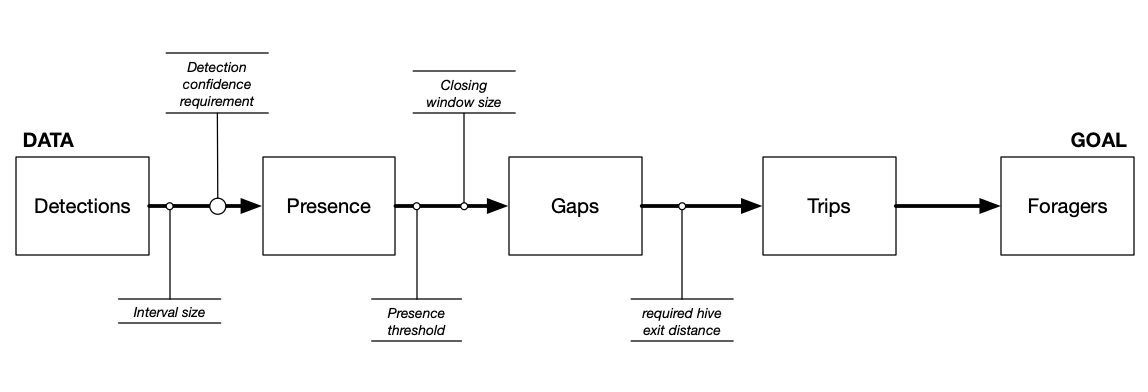
\includegraphics[width=1.0\textwidth]{funnel-params}
\caption[funnel-params]{Visualization of the abstraction steps, with some of the parameters involved in creating them. Emphasized is the only parameter that has been reliably tested for a better value}
\label{fig:funnel-params}
\end{figure}




\section{Contributing abstractions}

While unsuccessful in detecting forager transitions, I'm contributing the concepts of Presence and Gaps, along with the code for computing them and the idea of generating those concepts often and saving well. I hope that will genuinely have a positive influence on future investigations, perhaps also involving the foraging question.


%!TEX root = ../thesis.tex
%*******************************************************************************
%*********************************** Fourth Chapter *****************************
%*******************************************************************************

\chapter{Future work}  %Title 

\ifpdf
    \graphicspath{{Chapters/Chapter6/Figs/Raster/}{Chapters/Chapter6/Figs/PDF/}{Chapters/Chapter6/Figs/}}
\else
    \graphicspath{{Chapters/Chapter6/Figs/Vector/}{Chapters/Chapter6/Figs/}}
\fi


%********************************** %First Section  **************************************
\section{Direct continuation}

As hinted at in previous sections, I could see a path to reliably identifying foragers based on the data at my disposal. While I am certain Trips cannot be identified accurately, I can imagine even a very rudimentary classifier for Trips could be enough to identify foragers, as all that it's needed is for the spike in trips to be noticable. For that, perhaps identifying as little as 10\% of Trips would suffice (provided they are more or less uniformly distributed among real Trips). This is the main reason I believe this approach could still be valid, even if it failed for my attempt.

A rudimentary classifier that would label ever Gap as a Trip or Not Trip could conceivably be trained by human labor in analyzing videos. This would not work if they were generated from the same set of Gaps that the 200 analyzed by me, but Gaps can easily be filtered to increase the likelyhood of finding Trips among them.

Filters could include:
\begin{itemize}
 \item time-of-day (foraging is a daily activity
 \item camera (only cameras 1 and 2 have access to the exit)
 \item exit distance (only disappearances near to the exit can be Trips)
\end{itemize}

If the likelyhood for the manual observer to find a gap is high enough (maybe about 20-30\% or more), this seems like a viable option of creating enough labeled examples to train (for example) a Random Forest classifier.


\section{Other ways of getting a labeled dataset}

That being said, there might be cheaper and more reliable ways of creating such labeled dataset. Two that come to mind (that have alread beed implemented in various experiments) are RFID tags and exit 
cameras. Out of this total of three approaches, I would lean toward exit cams as the easiest to bring to life. It requires much less labor than analyzing videos or tagging every bee with an RFID chip, it's also probably cheaper that the latter. The only consideration here would be that it's not trivial to install cameras in a way that ensures a bee's tag will always be recognized as she exits. Even the smallest tube is a 3D space and would be prone to the same problems that the in-hive cameras are prone to: tags oriented at unreadable angles or occluded by other bees. Ideally, three or four cameras would observe the exit, so that no orientation of the bee would make the tag unreadable. To limit occlusions, the tube should be as tight as possible, the lower limit being that an exiting bee can pass a bee trying to enter. The tube should also have enough length so that if occlusions appear, they are made up for by the cameras detecting occluded bees later.

Being able to observe bees exit the hive would be a much more reliable way of building up a forager database. That could of course be used directly for analysis, but it would be beneficial to use it to train a classifier - this way, future or independent iterations of BeesBook could perform analysis on Foragers without installing exit cameras.










% ********************************** Back Matter *******************************
% Backmatter should be commented out, if you are using appendices after References
%\backmatter

% ********************************** Bibliography ******************************
\begin{spacing}{0.9}

% To use the conventional natbib style referencing
% Bibliography style previews: http://nodonn.tipido.net/bibstyle.php
% Reference styles: http://sites.stat.psu.edu/~surajit/present/bib.htm

\bibliographystyle{apalike}
%\bibliographystyle{unsrt} % Use for unsorted references  
%\bibliographystyle{plainnat} % use this to have URLs listed in References
\cleardoublepage
\bibliography{End-sections/References/references} % Path to your References.bib file


% If you would like to use BibLaTeX for your references, pass `custombib' as
% an option in the document class. The location of 'reference.bib' should be
% specified in the preamble.tex file in the custombib section.
% Comment out the lines related to natbib above and uncomment the following line.

%\printbibliography[heading=bibintoc, title={References}]


\end{spacing}

% ********************************** Appendices ********************************

\begin{appendices} % Using appendices environment for more functunality

%!TEX root = ../thesis.tex
% ******************************* Thesis Appendix A ****************************
\chapter{How to install \LaTeX} 

\section*{Windows OS}

\subsection*{TeXLive package - full version}
\begin{enumerate}
\item	Download the TeXLive ISO (2.2GB) from\\
\href{https://www.tug.org/texlive/}{https://www.tug.org/texlive/}
\item	Download WinCDEmu (if you don't have a virtual drive) from \\
\href{http://wincdemu.sysprogs.org/download/}
{http://wincdemu.sysprogs.org/download/}
\item	To install Windows CD Emulator follow the instructions at\\
\href{http://wincdemu.sysprogs.org/tutorials/install/}
{http://wincdemu.sysprogs.org/tutorials/install/}
\item	Right click the iso and mount it using the WinCDEmu as shown in \\
\href{http://wincdemu.sysprogs.org/tutorials/mount/}{
http://wincdemu.sysprogs.org/tutorials/mount/}
\item	Open your virtual drive and run setup.pl
\end{enumerate}

or

\subsection*{Basic MikTeX - \TeX~ distribution}
\begin{enumerate}
\item	Download Basic-MiK\TeX (32bit or 64bit) from\\
\href{http://miktex.org/download}{http://miktex.org/download}
\item	Run the installer 
\item	To add a new package go to Start >> All Programs >> MikTex >> Maintenance (Admin) and choose Package Manager
\item	Select or search for packages to install
\end{enumerate}

\subsection*{TexStudio - \TeX~ editor}
\begin{enumerate}
\item	Download TexStudio from\\
\href{http://texstudio.sourceforge.net/\#downloads}
{http://texstudio.sourceforge.net/\#downloads} 
\item	Run the installer
\end{enumerate}

\section*{Mac OS X}
\subsection*{MacTeX - \TeX~ distribution}
\begin{enumerate}
\item	Download the file from\\
\href{https://www.tug.org/mactex/}{https://www.tug.org/mactex/}
\item	Extract and double click to run the installer. It does the entire configuration, sit back and relax.
\end{enumerate}

\subsection*{TexStudio - \TeX~ editor}
\begin{enumerate}
\item	Download TexStudio from\\
\href{http://texstudio.sourceforge.net/\#downloads}
{http://texstudio.sourceforge.net/\#downloads} 
\item	Extract and Start
\end{enumerate}


\section*{Unix/Linux}
\subsection*{TeXLive - \TeX~ distribution}
\subsubsection*{Getting the distribution:}
\begin{enumerate}
\item	TexLive can be downloaded from\\
\href{http://www.tug.org/texlive/acquire-netinstall.html}
{http://www.tug.org/texlive/acquire-netinstall.html}.
\item	TexLive is provided by most operating system you can use (rpm,apt-get or yum) to get TexLive distributions
\end{enumerate}

\subsubsection*{Installation}
\begin{enumerate}
\item	Mount the ISO file in the mnt directory
\begin{verbatim}
mount -t iso9660 -o ro,loop,noauto /your/texlive####.iso /mnt
\end{verbatim}

\item	Install wget on your OS (use rpm, apt-get or yum install)
\item	Run the installer script install-tl.
\begin{verbatim}
	cd /your/download/directory
	./install-tl
\end{verbatim}
\item	Enter command `i' for installation

\item	Post-Installation configuration:\\
\href{http://www.tug.org/texlive/doc/texlive-en/texlive-en.html\#x1-320003.4.1}
{http://www.tug.org/texlive/doc/texlive-en/texlive-en.html\#x1-320003.4.1} 
\item	Set the path for the directory of TexLive binaries in your .bashrc file
\end{enumerate}

\subsubsection*{For 32bit OS}
For Bourne-compatible shells such as bash, and using Intel x86 GNU/Linux and a default directory setup as an example, the file to edit might be \begin{verbatim}
edit $~/.bashrc file and add following lines
PATH=/usr/local/texlive/2011/bin/i386-linux:$PATH; 
export PATH 
MANPATH=/usr/local/texlive/2011/texmf/doc/man:$MANPATH;
export MANPATH 
INFOPATH=/usr/local/texlive/2011/texmf/doc/info:$INFOPATH;
export INFOPATH
\end{verbatim}
\subsubsection*{For 64bit OS}
\begin{verbatim}
edit $~/.bashrc file and add following lines
PATH=/usr/local/texlive/2011/bin/x86_64-linux:$PATH;
export PATH 
MANPATH=/usr/local/texlive/2011/texmf/doc/man:$MANPATH;
export MANPATH 
INFOPATH=/usr/local/texlive/2011/texmf/doc/info:$INFOPATH;
export INFOPATH

\end{verbatim}



%\subsection{Installing directly using Linux packages} 
\subsubsection*{Fedora/RedHat/CentOS:}
\begin{verbatim} 
sudo yum install texlive 
sudo yum install psutils 
\end{verbatim}


\subsubsection*{SUSE:}
\begin{verbatim}
sudo zypper install texlive
\end{verbatim}


\subsubsection*{Debian/Ubuntu:}
\begin{verbatim} 
sudo apt-get install texlive texlive-latex-extra 
sudo apt-get install psutils
\end{verbatim}

%!TEX root = ../thesis.tex
% ******************************* Thesis Appendix B ********************************

\chapter{Installing the CUED class file}

\LaTeX.cls files can be accessed system-wide when they are placed in the
<texmf>/tex/latex directory, where <texmf> is the root directory of the user’s \TeX installation. On systems that have a local texmf tree (<texmflocal>), which
may be named ``texmf-local'' or ``localtexmf'', it may be advisable to install packages in <texmflocal>, rather than <texmf> as the contents of the former, unlike that of the latter, are preserved after the \LaTeX system is reinstalled and/or upgraded.

It is recommended that the user create a subdirectory <texmf>/tex/latex/CUED for all CUED related \LaTeX class and package files. On some \LaTeX systems, the directory look-up tables will need to be refreshed after making additions or deletions to the system files. For \TeX Live systems this is accomplished via executing ``texhash'' as root. MIK\TeX users can run ``initexmf -u'' to accomplish the same thing.

Users not willing or able to install the files system-wide can install them in their personal directories, but will then have to provide the path (full or relative) in addition to the filename when referring to them in \LaTeX.

\end{appendices}

% *************************************** Index ********************************
\printthesisindex % If index is present

\end{document}
